% !TEX encoding = UTF-8 Unicode

\documentclass[12pt,a4j,titlepage]{ltjsarticle}
\usepackage{semi}
\usepackage{here}
\usepackage{listings}

% \title{}
% \author{}
% \date{}

\begin{document}

\begin{titlepage}
  \begin{center}
  
    \vspace*{20truept}
    
    {\LARGE 2024年度 卒業論文} 
    
    \vspace*{75truept}
    
    {\Huge  タイトル} %論文タイトル

    \vspace{10truept}

    {\Huge } %論文タイトル 長い場合 改行1

    \vspace{10truept}

    {\Huge } %論文タイトル 改行2

    \vspace{85truept}
    
    {\LARGE 指導教員 須田 宇宙 准教授}
    
    \vspace{60truept}
    
    {\LARGE 千葉工業大学 情報ネットワーク学科}
    
    \vspace{15truept}
    
    {\LARGE 須田研究室}
    
    \vspace{70truept}
    
    {\LARGE 2132100 氏名 中野 星花 } % 氏名は消さない 学生番号 氏名 名前

    \vspace{70truept}
    
  \end{center}
  \begin{flushright}

    {\LARGE 提出日 2024年1月17日}
  
  \end{flushright}
\end{titlepage}

\setcounter{tocdepth}{3}
% 目次の出力
\tableofcontents

\clearpage

% 表目次
\listoftables
% 図目次
\listoffigures
\clearpage

\section{緒言}\label{緒言}
%背景


%問題点


%目的


\clearpage

\section{学習について}
近年,労働人口の減少,グローバル化の進展や技術革新等により,現代社会の構造や雇用環境が急速に変化している.
このような時代背景から,教育を通して変化に対応し協力して課題を解決する力,情報を判断し再構成して新たな価値を生み出す力,複雑な状況で目的を見直す力が求められている.
また,令和3年1月の中央教育審議会の答申では,「主体的・対話的で深い学び」の実現に向けて,個別最適な学びと協働的な学びを「令和の日本型学校教育」の姿として提唱している.

個別最適な学びとは,ICT環境を活用した個に応じた指導の充実を図る.
その際,個々の興味・関心・意欲等を踏まえた指導や,学習者自身が学習状況を把握し,主体的に学習を調整することができるよう促すことが求められる.

協働的な学びとは,探求的な学習や体験活動等を通じ,他者と協働しながら必要な資質・能力を育成する.

\subsection{個別学習について}
ICTを活用することにより学びの場において,教員による一斉指導に加え,学習者個人の能力や特性に応じた教材を用いた主体的な学習が可能になった.
個に応じた学習では,個人の理解度や誤答傾向に応じた問題の作成や,教員が学習履歴の管理などの支援を行うことが容易になった.

一方で,個別学習で基礎知識を習得した後,その知識を深めるためには,他者との交流や意見交換を通じて多角的に学ぶ機会が必要となる.

\subsection{探求学習について}
探求学習では,「変化の激しい社会に対応して,探求的な見方・考え方を働かせ,横断的・総合的な学習を行うことを通して,よりよく課題を解決し,自己の生き方を考えていくための資質・能力を育成することを目標にしている」.
探求の過程において,課題の発見と解決に取り組むという過程がある.
しかし問や課題は,学習者が持っている知識や経験だけでは生まれないこともある.
従って,他者の考えを自己の常識に照らして違和感を抱く問題があることなどを発見し,課題発見につなげる機会が必要になる.
また,課題解決能力は,学習者自身が必要な知識を取捨選択し,整理し,すでに持っている知識や体験と結びつけながら身につけることができる.

\clearpage

\subsection{協働学習について}
協働学習とは「主体的で自律的な学びの構え,確かで幅広い知的習得,仲間と共に課題解決に向かうことのできる対人技能,さらには,他者を尊重する民主的な態度,といった『学力』を効率的に身につけていくための『基本的な考え方』」を指す.

学習者が主体的で自律的な学力をつけることは,一対多の講義形式のような,学習者が受け身で学ぶ授業では困難である.
なぜなら受け身の学習では,知識や技能が,教師から学習者へと受け渡しされ,授業の中で学習者にどのような学びが起こっているのかは重要ではなく,テストなどの結果に関心が置かれるからである.

%なぜなら の書き方があんまよくないかも??

従って,学習者自身が授業で教わった知識を主体的に深めるために,他者と協働しながら問題解決に挑むことが必要になる.
協働学習では,学習者同士が意見を交換し,異なる視点や考え方に触れることで,多様な理解が促進される.
これにより,個人の思考が広がり,より豊かな学びが実現することが研究で明らかになっている.\cite{suzuki}
また,仲間と共に学ぶ過程で,コミュニケーション能力や対人関係のスキルが育まれ,他者を尊重する態度が培われる.

このように,協働学習は,学力向上だけでなく,社会で求められる幅広い能力を効果的に育成するための重要な学習方略である.

一方で,対話相手によって,学力の向上に繋がらない場合がある.

\subsection{大学教育で育成すべき能力}
現代社会は,生産年齢人口の減少や技術革新等により,社会構造や雇用環境が急速に変化している.
従って,今後どのように社会が変化していくかを予測することが困難になっている.
そのことから,一人一人が持続可能な社会を支えることが求められており,その能力を生かして個人と社会の成長につながる新たな価値を生み出していくことが必要である.
このことより文部科学省は,高度の専門知識を備えた人材やグローバル化に対応した人材の育成を目指しており,課題探求能力の他に学士力として専門的知識,汎用的能力,人材形成を大学で育成することを2012年から求められている.

\subsection{知識の体系化について}
\subsubsection{概要}
知識の体系化とは,学習によって習得した知識同士が関連している状態を指す.
体系化によって,学習内容の全体像を把握することになるため,問題や課題が生じた際に,多くの知識を解決に使用することが出来る.
知識同士が関連している状態を図\ref{fig:tisiki_doai}に示す.

\begin{figure}[!htb]
  \centering
  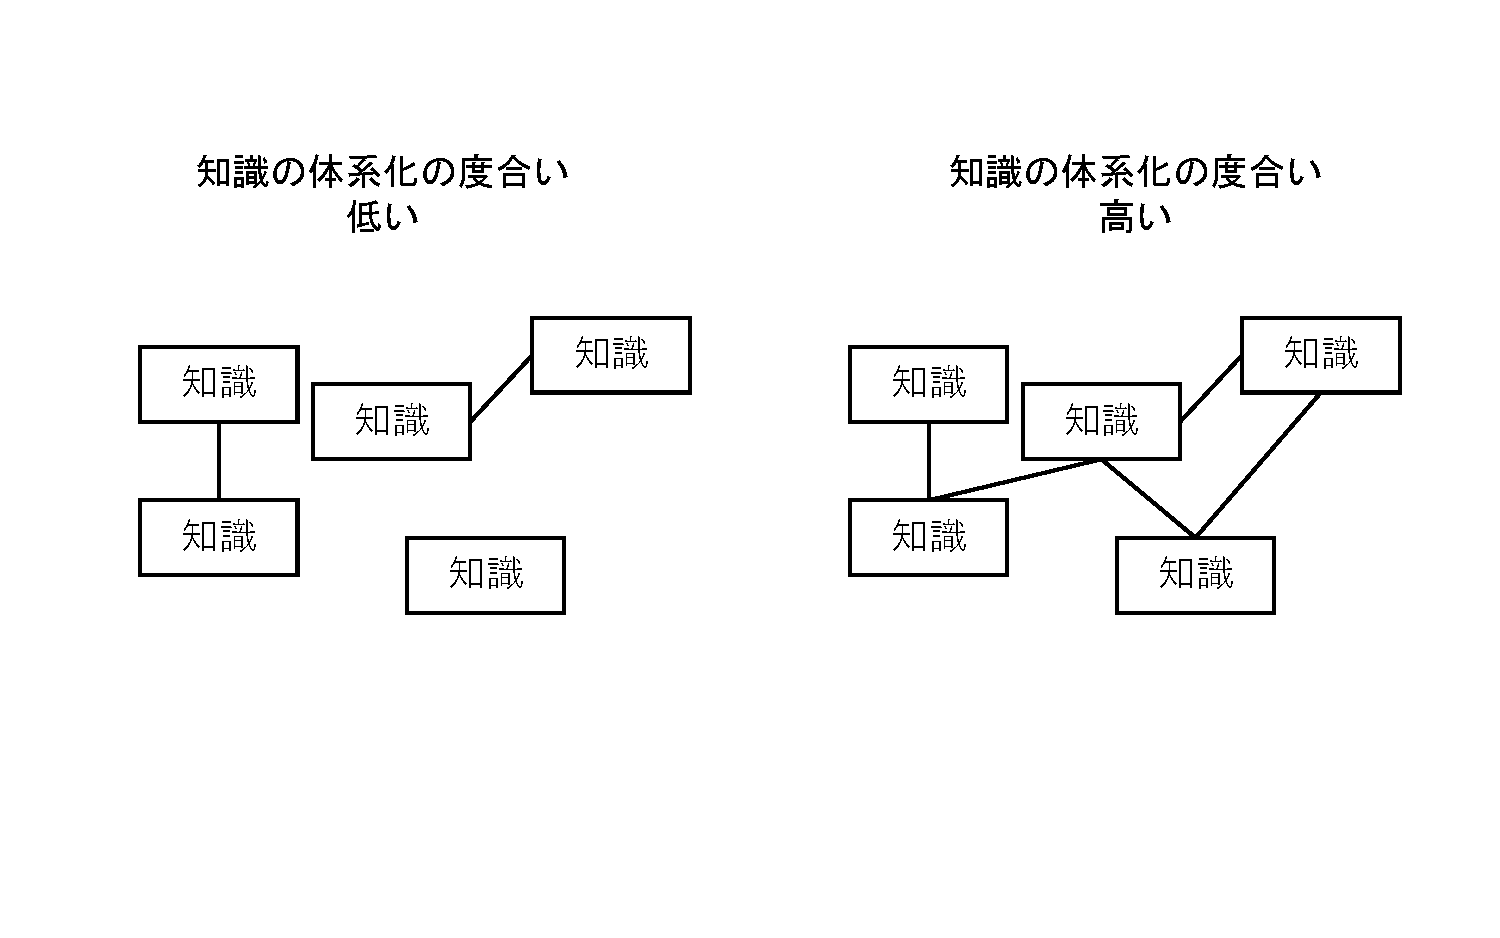
\includegraphics[width=15cm]{tisiki_doai.pdf}
  \caption{知識の体系化の度合い}
  \label{fig:tisiki_doai}
\end{figure}


\subsubsection{学習における体系化の重要性}
学習において体系化は,学習内容を整理し,論理的な順序や構造に基づいて組み立てることで,知識の定着を助け,応用力や問題解決能力を向上させるために有効である.


%\subsection{対話相手の違いと体系化への影響}
%対話相手の違いとは,主に相手との親密度,相手の知識量,相手の知識の体系化の程度が挙げられる.

%親しい相手との対話では,親しくない相手と比較すると,自由な発言と試行錯誤が促される点がある.カジュアルに意見を交わしやすいことによる違いが生じる.

%相手が自分より知識量が多い場合,質問を通じて理解を深める機会が多いが,議論が一方的になり,主体的な思考を妨げる可能性がある.一方,自分より相手の知識量が少ない場合,相手に教える立場になりやすいため,分かりやすく伝えるために,単純化や具体例を交えることで理解が深まる機会が多い.しかし,この場合も議論が一方的になりやすいという問題がある.


\section{演習・実習について}
大学のカリキュラムに,演習・実習を体系的に配置することで,自主的な姿勢で課題に取り組むように指導を実施している.

また,思考・判断のプロセスを説明するためのプレゼンテーション能力やコミュニケーション能力,グループでの共同作業を適確に実行し,協力関係をつくり上げていく能力を育成することが目的である.

\subsection{ネットワーク管理実習}
\subsection{概要}
ネットワーク管理実習は,第6セメスターに開講されている科目である.
この授業の目的は,インターネットの普及に伴い,各種組織から一般家庭に至るまで幅広く利用されているTCP/IPを基盤としたローカルエリアネットワーク(LAN)の管理に必要なスキルを習得することにある.
しかし,LANの設計や構築を担う技術者は必ずしも十分に確保されているとは言えず,こうした状況に対応するためには実践的な学習の場が求められている.
このような背景を踏まえ,本実習では,LANの構成単位であるサブドメインの設計・構築を行い,LANの構築に応用することで,LAN管理に必要な実践的スキルの習得を目指す.
表\ref{tb:kougi}に各週の授業内容を示す.

%表1
\begin{table}[htbp]
  \caption{ネットワーク管理実習の学習内容}
  \begin{center}
\begin{tabular}{ll}\hline
               週 & 授業内容 \\ \hline
               1 & ガイダンス\\
               2 & ユーザ管理 アクセス権\\
               3 & シェルの基本\\
               4 & TCP/IPについて\\
               5 & IPアドレッシング手法\\
               6 & ルーティングとルータ\\
               7 & パッケージのインストール\\
               8 & 名前解決の仕組み\\
               9 & DNSを利用した問い合わせの仕組み\\
              10 & DNSを利用した問い合わせの仕組み\\
              11 & メール配信の仕組み SMTPサーバの構築\\
              12 & Webサーバの構築\\
              13 & 期末テスト\\
              \hline
               \end{tabular}
               \end{center}
               \label{tb:kougi}
               \end{table}

\subsubsection{Unixコマンド}
Unixは,1969年にAT\&Tのベル研究所で開発が進められたOSであり,1970年代には大学や研究所などで利用され始めた.シンプルな設計と効率性の高さから移殖・拡張が繰り返され,類似OSであるLinuxを含めてUNIX系OSと呼ばれ今でも利用されている.
Unix系OSは専用の入力画面にコマンドを打ち込んで操作するCUI方式が採用されており,ファイルの操作や情報の取得などの作業をする際に使用される.


\subsubsection{ルーティング}
インターネットでは,IPアドレッシングに基づき割り当てられたネットワークが互いに接続されている.
これらのネットワーク間でパケットを転送することをルーティングといい,この中継を行う装置をルータという.
ここで,ルータは接続するネットワークの数だけネットワークインタフェースを持つ.

また,離れたホストへ通信する際に多くのルータを経由する.
この順路のことをルートという.
そのため,ルータはパケットを中継する際にどのルータへパケットを渡せば目的のホストにパケットが届けられるかを知る必要がある.
この情報を経路情報という.
経路情報には目的のネットワークの存在する方向(インタフェース)とその優先度が書かれたルーティングテーブルを利用する.

\subsubsection{名前解決}
名前解決とは,IPアドレスとドメイン名であるFQDNを相互に変換することを指す.
この時,FQDNからIPアドレスを調べることを「正引き名前解決」と呼び,IPアドレスからFQDNを調べることを「逆引き名前解決」という.
また,この仕組みを提供するサーバをDNSサーバという.

\subsubsection{SMTPサーバ}
SMTPサーバとは,メール送信の際に必要となるサーバーである.
メールを送信の命令を受け取ったSMTPサーバーは,送信メールを,送信先メールアドレスを管理するSMTPサーバーまで送る.




\section{OSI参照モデル}
\subsection{概要}
OSI参照モデルとは,コンピュータが通信するために利用するネットワークの機能を7つの階層(レイヤー)に分類して,機能を分割することで,複雑なネットワークプロトコルを単純化したモデルである.
最初のネットワークの実装では,各メーカーや組織独自の通信プロトコルを用いていた.
しかし,このモデルを用いるようになったことで,ネットワークの設計が体系化され,標準化が進展した.
また,データをやり取りする際,機種や通信方式といった様々な違いを考慮しなければならない.
データの送信側と受信側のコンピュータのプログラムがあらかじめ決められたマニュアル(プロトコル)に沿って通信し,OSI参照モデルに準拠するよう各種プロトコルが作られている.

\subsubsection{階層化}
アプリケーション層は,ユーザーが操作するアプリケーションの中で通信に関係する具体的な機能についての仕様や手順を定めて過程で
ファイル転送や電子メール,遠隔ログインなどを実現するためのプロトコルがある.

プレゼンテーション層では,データの表現形式を定義する.
具体的に,アプリケーションが扱う情報を通信に適したデータ形式にしたり,また下位層から来たデータを上位層が処理できるデータ形式にするなどがある.

セッション層は,通信プログラムの確立や切断,転送するデータの切れ目の設定など一連の手順(セッション)を定義する.

トランスポート層は,宛先のアプリケーションにデータを確実に届ける際,通信の品質をコントロールする層である.
信頼性重視やリアルタイム性重視など,用途に応じてプロトコルを使い分ける.
通信を行う両端のノード(機器)だけで処理され,途中のルーターでは処理されない.

ネットワーク層は,宛先までデータを届ける役割を持つ.
宛先が複数のネットワークアドレスでつながった先にある場合には,アドレス体系決めや,通信経路選択(ルーティング)の役割を持つ.

データリンク層は,物理層で直接接続されたノード間での通信を可能にする.
0と1の数字の列を意味のあるかたまり(フレーム)に分けて,相手に伝える.

物理層は,ビットの列(0と1の数字の列)を物理的な信号に変換し,実際の通信媒体を通じて送信する.

これらのそれぞれ独立した役割を持つ7つの階層が,互いに連携して通信を実現している.

\subsection{各層のデータ通信}
送信側の各階層でデータが処理される際,上位の階層から受け取ったデータに,その階層独自の情報(ヘッダ)を付加して下位の階層に引き渡す.
ヘッダには,その階層での通信制御やエラー検出,送信先情報など,通信を適切に管理するための情報が含まれている.
また,データリンク層ではデータの末尾にトレーラを付加する場合がある.
トレーラには,データが伝送中に損傷していないかを確認するためのエラー検出用の情報が含まれる.
一方で,受信側ではこれが逆順に処理され,各階層で対応するヘッダやトレーラが解析されることで,元のデータがアプリケーション層に復元される.

\section{研究概要}
\subsection{対話学習の内容}

本研究で用いた対話学習の内容は,ネットワーク管理実習の第11回の課題11-2-4. 「ドメイン間の電子メール送受信確認」の実施にあたり,エラーが生じたため,解決のための対話である.

ネットワーク管理実習の講義を受講した4人の学生とシステムエラーの原因を対話をしながら一緒に考える.ここで,被験者を学習者A,実験者を学習者Bとする.

また,講義で学んだ知識が体系化されたかどうか確認するためのインタビューを行った.

\section{評価}

この章では対話学習の評価について述べる.
評価項目として,学習者Bの知識の体系化の程度が学習者Aの学習に与える影響について調べる.


\subsection{インタビュー内容}
学習者Bにインタビューを行った.
インタビューの内容は表\ref{tb:interview}に応じた質問を行った.

\begin{table}[htbp]
\begin{center}
\caption{インタビュー結果 学習者Bの知識の体系化の度合い:低い}
\begin{tabular}{|p{8cm}|p{8cm}|}
\cline{1-2}
実験者 (質問)  & 被験者 Aさん   \\ \cline{1-2}
対話学習を終えて,知識が体系化されたと感じましたか.   & はい.       \\ \cline{1-2}
具体的にどの知識が体系化されましたか.                 & メールを送る仕組みについてちゃんと整理できた. 特に,上流ネットワークにメールを送れないから,ルーターの設定に問題がある点がちゃんと結びついた.   \\ \cline{1-2}
普段の授業や学習で誰かと話すことで知識が体系化された経験はありますか. & はい.         \\ \cline{1-2}
普段の授業や学習に対話学習を用いることは必要だと思いますか.      & 知識を習得した後じゃないと対話が活発にならないため,座学には必要だとは思わない.      \\ \cline{1-2}
\end{tabular}
\end{center}
\label{tb:interview}
\end{table}

\clearpage

\begin{table}[htbp]
\begin{center}
\caption{インタビュー結果 学習者Bの知識の体系化の度合い:なし}
\begin{tabular}{|p{8cm}|p{8cm}|}
\cline{1-2}
実験者 (質問)  & 被験者 Bさん   \\ \cline{1-2}
対話学習を終えて,知識が体系化されたと感じましたか.   & 感じたが,対話によって体系化ができたというより,調べたからなのではないかとも思った.       \\ \cline{1-2}
具体的にどの知識が体系化されましたか.                 & ルーターの設定の必要性について,メールが上流ネットワークに送れないというエラーを解決することを考えていくことでちゃんと理解できた.   \\ \cline{1-2}
普段の授業や学習で誰かと話すことで知識が体系化された経験はありますか. & はい.         \\ \cline{1-2}
普段の授業や学習に対話学習を用いることは必要だと思いますか.      & 学習の目的が知識の獲得であったらいらないと思うが,結局知識単体では役に立たないため,対話で知識が体系化されるのなら必要になると思う.      \\ \cline{1-2}
\end{tabular}
\end{center}
\label{tb:interview}
\end{table}

\clearpage


\begin{table}[htbp]
\begin{center}
\caption{インタビュー結果 学習者Bの知識の体系化の度合い:低い}
\begin{tabular}{|p{8cm}|p{8cm}|}
\cline{1-2}
実験者 (質問)  & 被験者 Cさん   \\ \cline{1-2}
対話学習を終えて,知識が体系化されたと感じましたか.   & はい.       \\ \cline{1-2}
具体的にどの知識が体系化されましたか.                 & メールを送る上で必要になる知識やシステムの全体像について分かった.また,ルーターの設定について実はちゃんと理解できていなかったことが対話によって分かった.   \\ \cline{1-2}
普段の授業や学習で誰かと話すことで知識が体系化された経験はありますか. & はい.         \\ \cline{1-2}
普段の授業や学習に対話学習を用いることは必要だと思いますか.      & 実はちゃんと理解できていない知識について,対話などのアウトプットで明確になるため,座学でも知識を体系化させる機会は必要だと思う.      \\ \cline{1-2}
\end{tabular}
\end{center}
\label{tb:interview}
\end{table}

\clearpage


\begin{table}[htbp]
\begin{center}
\caption{インタビュー結果 学習者Bの知識の体系化の度合い:なし}
\begin{tabular}{|p{8cm}|p{8cm}|}
\cline{1-2}
実験者 (質問)  & 被験者 Dさん   \\ \cline{1-2}
対話学習を終えて,知識が体系化されたと感じましたか.   & 時間はかかってしまったが,体系化されたと感じた.     \\ \cline{1-2}
具体的にどの知識が体系化されましたか.                 & 実習中は,知識を習得しながら作業することに集中していたため,知識の体系化をできていなかったことが分かった.また,授業資料に沿って作業していたため,エラーが起きることがなかったため,エラーが起きた時にシステムの全体像を改めて考え,体系化された.   \\ \cline{1-2}
普段の授業や学習で誰かと話すことで知識が体系化された経験はありますか. & はい.         \\ \cline{1-2}
普段の授業や学習に対話学習を用いることは必要だと思いますか.      & 知識を誰かに説明するときに定着するようになったため,対話学習は活用する機会はあっていいと思う.      \\ \cline{1-2}
\end{tabular}
\end{center}
\label{tb:interview}
\end{table}

\clearpage


\subsection{考察}
\subsection{今後の課題}



\clearpage



\section{謝辞}
本研究の遂行及び本論文の作成にあたり,須田研究室の仲間に多くの手助けを頂きました,深く感謝の意を表します.そして,本論文の作成にあたり多大なる御指導及び御助言を頂きました,須田宇宙准教授に深く感謝の意を表します.

\clearpage

%参考文献
\begin{thebibliography}{99}
\bibitem{TCP/IP} (1994) 竹下隆史・松山公保・荒井透・苅田幸雄: ``マスタリングTCP/IP 入門編第5版''

\cite{inagaki}
\cite{TCP/IP}
\cite{suzuki}

\end{thebibliography}
\bibliographystyle{jplain}
\bibliography{ronbun}

\section{付録}

\begin{figure}[!htb]
  \centering
  \includegraphics[width=15cm]{実験用スライド.pdf}
  \caption{実験に用いた資料}
  \label{fig:jikkenn}
\end{figure}

\end{document}
